\documentclass[12pt]{report}
\usepackage{amsthm}
\usepackage{amssymb}
\usepackage{amsmath}
\usepackage{listings}
\usepackage{graphicx}
\usepackage{float}
\usepackage{xcolor}
\usepackage{hyperref}
\usepackage{multicol}
\usepackage{enumitem}
\usepackage[italian]{babel}
\usepackage{titlesec}
\usepackage{listings}
\usepackage{xcolor} % Per i colori

\hypersetup{
    colorlinks=true,
    linkcolor=black,
    filecolor=magenta,      
    urlcolor=blue,
    pdftitle={Relazione Prenotazioni Mediche},
    pdfpagemode=FullScreen,
}

\setlength{\parindent}{0pt}
\setlength{\parskip}{5pt}
\titlespacing{\section}{0pt}{0.5em}{0.3em}
\titlespacing{\subsection}{0pt}{0.8em}{0.4em}

\begin{document}
    \renewcommand{\labelenumii}{\arabic{enumi}.\arabic{enumii}}
    \renewcommand{\labelenumiii}{\arabic{enumi}.\arabic{enumii}.\arabic{enumiii}}
    \renewcommand{\labelenumiv}{\arabic{enumi}.\arabic{enumii}.\arabic{enumiii}.\arabic{enumiv}}

    \title{Relazione \\Prenotazioni Mediche\\Ingegneria del software}
    \author{D. Quattrociocchi (2024239) - G.Sepe (1983219)\\L. Mastromattei (1958925)}
    \date{\today}
    
    \maketitle
    \tableofcontents
    \newpage
        
    
    \chapter{Descrizione generale}
    
   Si intende progettare una piattaforma digitale per la gestione delle prenotazioni mediche, che consenta ai pazienti, previa registrazione, di prenotare visite specialistiche, ai medici di vedere i loro impegni e agli amministrativi di gestire i vari appuntamenti.

Un paziente può registrarsi sulla piattaforma fornendo le seguenti informazioni personali: nome, cognome, codice fiscale, data di nascita, indirizzo email, numero di telefono e indirizzo completo, composto da via, numero civico, CAP, città e provincia. Ad un potenziale paziente è possibile utilizzare la piattaforma, anche senza registrazione, per effettuare una ricerca dei medici disponibili. Ma solamente una volta completata la registrazione, il paziente avrà la facoltà di prenotare una visita medica, e in seguito lasciare un feedback relativo alla propria esperienza esprimendo due valutazioni numeriche, da 0 a 5, rispettivamente sulla soddisfazione complessiva e sulla puntualità del servizio ricevuto. La piattaforma consente inoltre ai pazienti di accedere alla cronologia delle prenotazioni effettuate.

Per quanto riguarda i medici, questi una volta inseriti nel sistema possono visualizzare sia le visite già svolte sia quelle ancora da svolgere. Inoltre, possono consultare le statistiche relative alla puntualità delle loro visite e alla soddisfazione dei propri pazienti. Al termine di ogni visita, il medico è tenuto a registrare sulla piattaforma il completamento della prestazione.

L'ultima entità che abbiamo realizzato è l'amministrativo, responsabile della supervisione della piattaforma e del corretto funzionamento di quest'ultima. L'amministrativo ha accesso a funzioni avanzate che gli permette di inserire un nuovo medico nel sistema e aggiungere periodi di indisponibilità o nuove specializzazioni acquisite ai medici già presenti. Inoltre agli amministratici è affidata la gestione delle richieste di prenotazione dei pazienti, che possono decidere se accettare o rifiutare; queste entreranno a far parte della cronologia delle prenotazioni gestite dall'amministrativo, che può essere poi da questo visualizzata.

    \newpage
    \chapter{Analisi del Software}
    \section{User Requirements}
    \subsection{Lista dei Requisiti}
    \begin{enumerate}
        \item Paziente non registrato
            \begin{enumerate}
                \item Ricerca medico
                    \begin{enumerate}
                        \item Specializzazione
                    \end{enumerate}
                \item Registrazione alla piattaforma
                    \begin{enumerate}
                        \item Nome
                        \item Cognome
                        \item Data di nascita
                        \item Codice Fiscale
                        \item Email
                        \item Recapito telefonico
                        \item Indirizzo
                            \begin{enumerate}
                                \item Via
                                \item Civico
                                \item CAP
                                \item Città
                                \item Provincia
                            \end{enumerate}
                    \end{enumerate}
            \end{enumerate}
        \item Paziente
            \begin{enumerate}
                \item Accesso cronologia prenotazioni
                \item Effettua prenotazione
                    \begin{enumerate}
                        \item ID medico
                        \item Specializzazione
                        \item Data
                    \end{enumerate}
                \item Lascia feedback
                    \begin{enumerate}
                        \item ID prenotazione conclusa
                        \item Voto soddisfazione
                        \item Voto puntualità
                    \end{enumerate}
                \item Ricerca medico
                    \begin{enumerate}
                        \item Specializzazione
                    \end{enumerate}
        \end{enumerate}
        \item Medico
            \begin{enumerate}
                \item Cronologia prestazioni
                \item Statistiche
                \item Termina prestazione
                    \begin{enumerate}
                        \item ID prenotazione accettata
                    \end{enumerate}
            \end{enumerate}
        \item Amministrativo
            \begin{enumerate}
                \item Inserisci medico
                    \begin{enumerate}
                        \item Nome
                        \item Cognome
                        \item Data di nascita
                        \item Codice Fiscale
                    \end{enumerate}
                \item Aggiungi indisponibilità medico
                    \begin{enumerate}
                        \item ID medico
                        \item Data inizio
                        \item Data fine
                    \end{enumerate}
                \item Aggiungi specializzazione medico
                    \begin{enumerate}
                        \item ID medico
                        \item Specializzazione
                    \end{enumerate}
                \item Accetta prenotazione
                \item Rifiuta prenotazione
                    \begin{enumerate}
                        \item Motivazione
                    \end{enumerate}
                \item Cronologia richieste prenotazioni
            \end{enumerate}
        
    \end{enumerate}
    
    \newpage
    
    \subsection{UML diagram}
    \begin{figure}[H]
        \centering
        \includegraphics[width=1\linewidth]{images/UML prenotazionimediche.png}
        \label{UML diagram}
    \end{figure}


    \subsection{Use-case diagram}
    \begin{figure}[H]
        \centering
        \includegraphics[width=1\linewidth]{images/Use-Case prenotazionimediche.png}
        \label{Use-case diagram}
    \end{figure}

    \newpage

    \section{System requirements}
    \subsection{Requisiti funzionali}
    \begin{enumerate}
        \item Paziente non registrato
            \begin{enumerate}
                \item Ricerca medico
                    \begin{enumerate}
                        \item Il sistema permette di ricercare i medici in base alla loro specializzazione, fornendo in output una lista di medici che la posseggono 
                    \end{enumerate}
                \item Registrazione alla piattaforma
                    \begin{enumerate}
                        \item Il sistema consente la registrazione tramite l'inserimento dei propri dati personali al paziente non registrato
                        \item Il nuovo utente deve essere inserito nel sistema sia come persona che come paziente
                    \end{enumerate}
            \end{enumerate}
        \item Paziente
            \begin{enumerate}
                \item Accesso cronologia prenotazioni
                    \begin{enumerate}
                        \item Il sistema permette all'utente di visualizzare la cronologia delle prenotazioni da lui effettuate che sono già state accettate
                        \item Il paziente vedrà sia le prenotazioni che sono già state concluse sia quelle che ancora devono avvenire
                    \end{enumerate}
                \item Effettuare prenotazioni
                    \begin{enumerate}
                        \item Ogni prenotazione deve essere effettuata da un paziente registrato che fornisce al sistema l'ID del medico con cui vuole effettuare la prenotazione, la specializzazione e data desiderate
                        \item Il sistema in automatico aggiunge alla richiesta di prenotazione l'ID del paziente che l'ha effettuata e quello dell'amministrativo che se ne occuperà
                    \end{enumerate}
                \item Lascia feedback
                    \begin{enumerate}
                        \item Il paziente una volta conclusa una visita può lasciare una valutazione da 0 a 5 sulla soddisfazione del cliente e sulla puntualità della visita; il sistema associa a questi due parametri l'ID del paziente e quello della prenotazione conclusa
                    \end{enumerate}
                \item Ricerca medico
                    \begin{enumerate}
                        \item Il sistema permette di ricercare i medici in base alla loro specializzazione, fornendo in output una lista di medici che la posseggono
                    \end{enumerate}
            \end{enumerate}
        \item Medico
            \begin{enumerate}
                \item Cronologia prestazioni
                    \begin{enumerate}
                        \item Il sistema permette ad ogni medico di visualizzare l'elenco sia delle prestazioni passato che di quelle ancora da svolgere
                    \end{enumerate}
                \item Statistiche
                    \begin{enumerate}
                        \item I medici possono visualizzare la media dei voti riguardanti la puntualità delle proprie visite e la soddisfazione dei pazienti, basate sui feedback di quest'ultimi
                    \end{enumerate}
                \item Termina prestazioni
                    \begin{enumerate}
                        \item Il sistema permette direttamente al medico di registrare il termine di ogni visita nel sistema non appena essa finisce
                    \end{enumerate}
            \end{enumerate}
        \item Amministrativo
            \begin{enumerate}
                \item Inserisci medico
                    \begin{enumerate}
                        \item Gli amministrativi  possono inserire all'interno del sistema nuovi medici, fornendo i suoi dati personali 
                        \item Anche in questo caso il nuovo utente deve essere inserito nel sistema sia come persona che come medico 
                    \end{enumerate}
                \item Aggiunta indisponibilità medico
                    \begin{enumerate}
                        \item Il sistema permette ad un amministrativo di aggiungere periodi d'indisponibilità ai medici fornendo il loro ID, la data d'inizio e la data di fine di questa
                        \item Ciò fa si che il sistema non accetta visite per il medico specificato in un determinato giorno e ora, se questo cade in un periodo  d'indisponibilità
                    \end{enumerate}
                \item Accetta prenotazione
                    \begin{enumerate}
                        \item Il sistema permette agli amministrativi di accettare le richieste di prenotazioni che gli sono state affidate
                    \end{enumerate}
                \item Rifiuta prenotazione
                    \begin{enumerate}
                        \item Il sistema permette agli amministrativi di rifiutare le richieste di prenotazioni che gli sono state affidate
                        \item In questo caso l'amministrativo aggiunte al rifiuto della richiesta di prenotazione anche una motivazione 
                    \end{enumerate}
                \item Cronologia richieste prenotazioni
                    \begin{enumerate}
                        \item Un amministrativo grazie a questa funzione è in grado di controllare la lista di prenotazioni da lui accettate che sono presenti nel sistema
                    \end{enumerate}
                \item Aggiungi specializzazione medico
                    \begin{enumerate}
                        \item Il sistema permette agli amministrativi di aggiungere una specializzazione ad ogni medico specificando l'ID di questo e una specializzazione, che ancora non possiede
                    \end{enumerate}
            \end{enumerate}
    \end{enumerate}

    \subsection{Requisiti non funzionali}
    \begin{enumerate}
        \item Il tempo medio di sessione di un client, cioè il tempo medio trascorso fra la connessione di un client ad un server e la sua disconnessione, deve essere inferiore a 10 secondi
        \item Il tempo medio di risposta del server ad una richiesta da parte di un client deve essere inferiore a 8 secondi
    \end{enumerate}

    \newpage
    \subsection{Architettura del sistema}
    Il sistema è stato progettato seguendo un approccio basato sulla separazione delle richieste ricevute. L'intero sistema viene infatti decentralizzato su quattro server che gestiscono richieste specifiche. Un server gestisce i \textbf{Pazienti non registrati}, uno è accessibile dai \textbf{Pazienti registrati}, un altro gestisce i \textbf{Medici} ed infine l'ultimo è accessibile  dagli \textbf{Amministrativi}.\\
    Tutti i server sono eseguiti in parallelo in modo da restituire lo stato di una richiesta.
     
    \begin{figure}[H]
        \centering 
        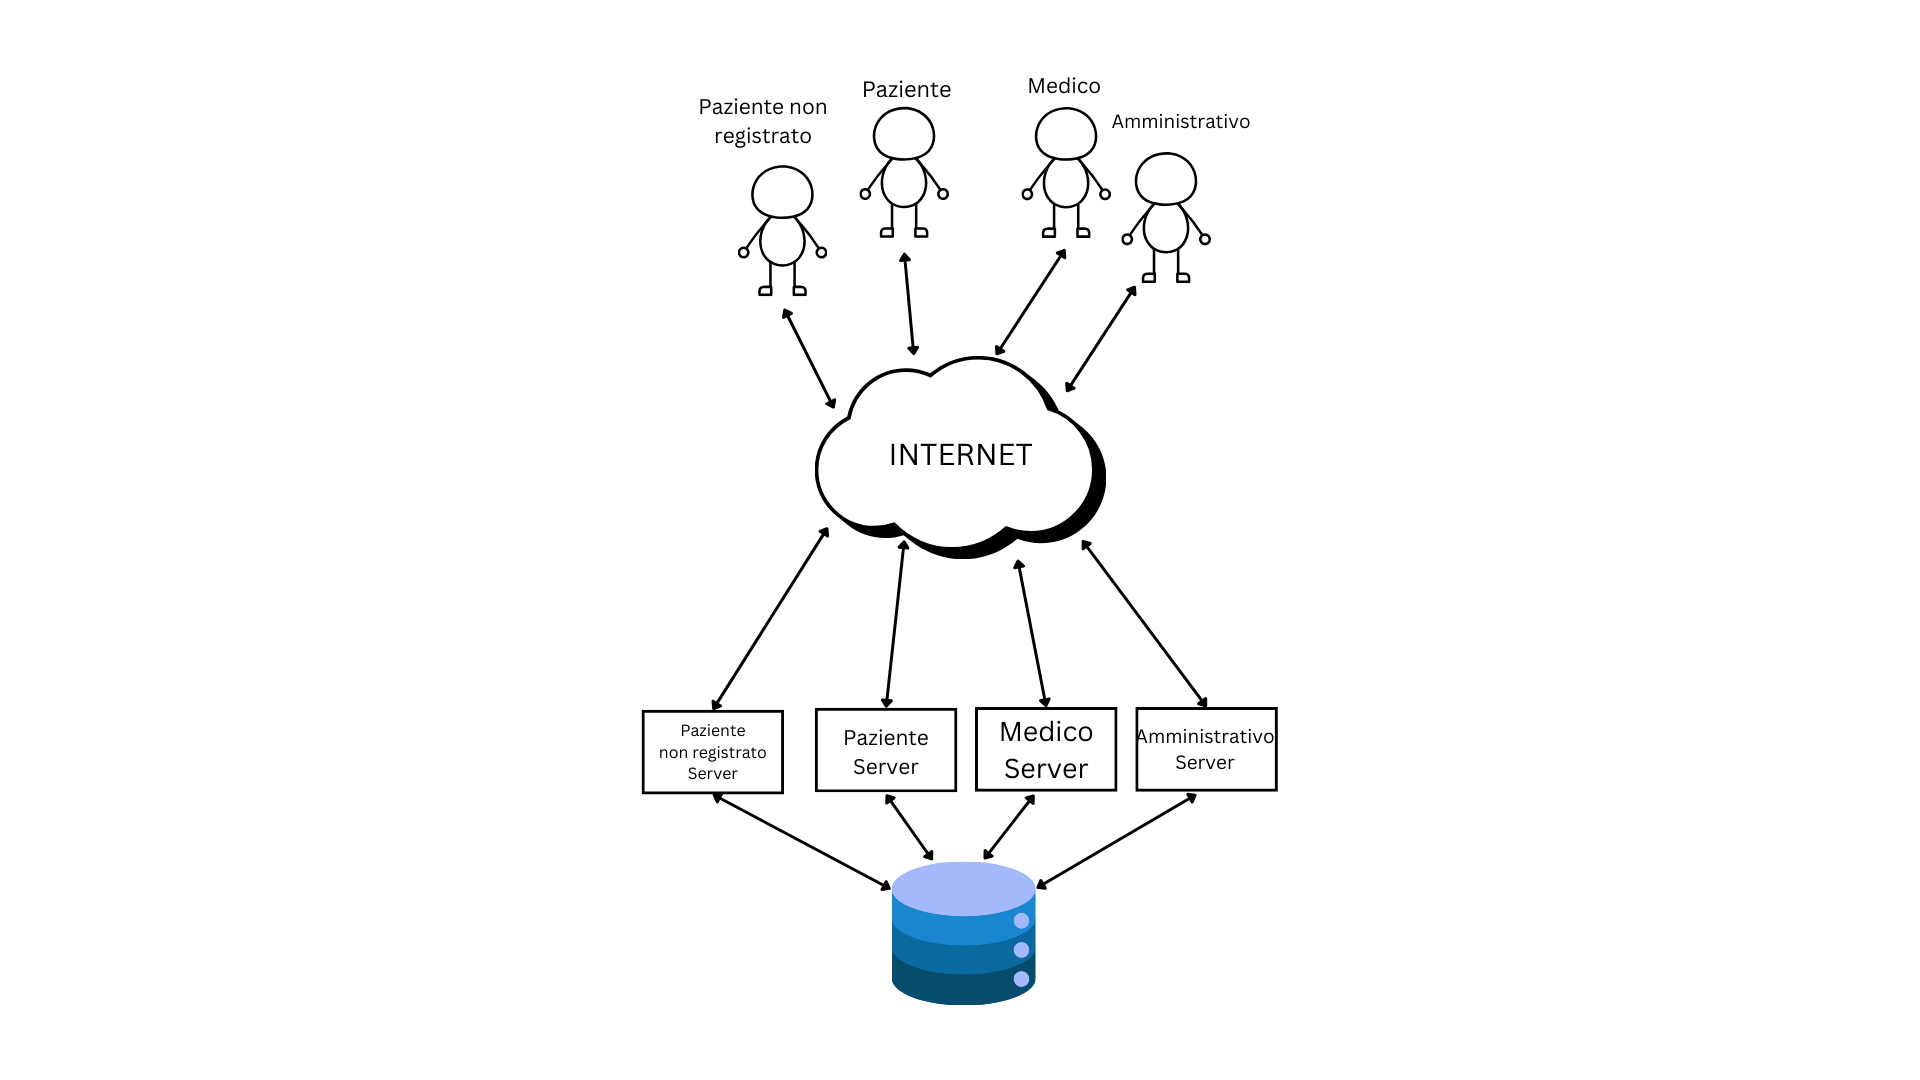
\includegraphics[width=1
        \linewidth]{images/Architettura.png}
        \label{Architettura}
    \end{figure}
    Ognuno dei quattro server viene a sua volta suddiviso in due componenti, un primo modulo denominato \textbf{Server}, addetto alla gestione delle richieste ricevute da ognuno degli utenti connessi al sistema e delle rispettive risposte, e un secondo modulo denominato \textbf{Handler}, addetto alla gestione dello smistamento delle richieste tra vari processi in esecuzione sul server stesso, inviando ogni richiesta tramite uno stream Redis al processo incaricato.\\ 
    Ciascuno di tali processi viene denominato \textbf{Funzione}. Ogni Funzione è una macchina a stati finiti che rimane in attesa di ricevere una richiesta da parte dell'Handler associato, per poi processare tale richiesta interagendo con il database ed infine restituire l'esito all'Handler.

    \subsection{Activity diagram}
    L'activity diagram rappresentato di seguito illustra l'invio di una richiesta da un client, la sua elaborazione e l'invio della risposta da parte del server. Questo processo è comune a tutti i server e a tutte le loro funzioni, indipendentemente dal tipo di richiesta effettuata dal client.

    \begin{figure}[H]
        \centering
        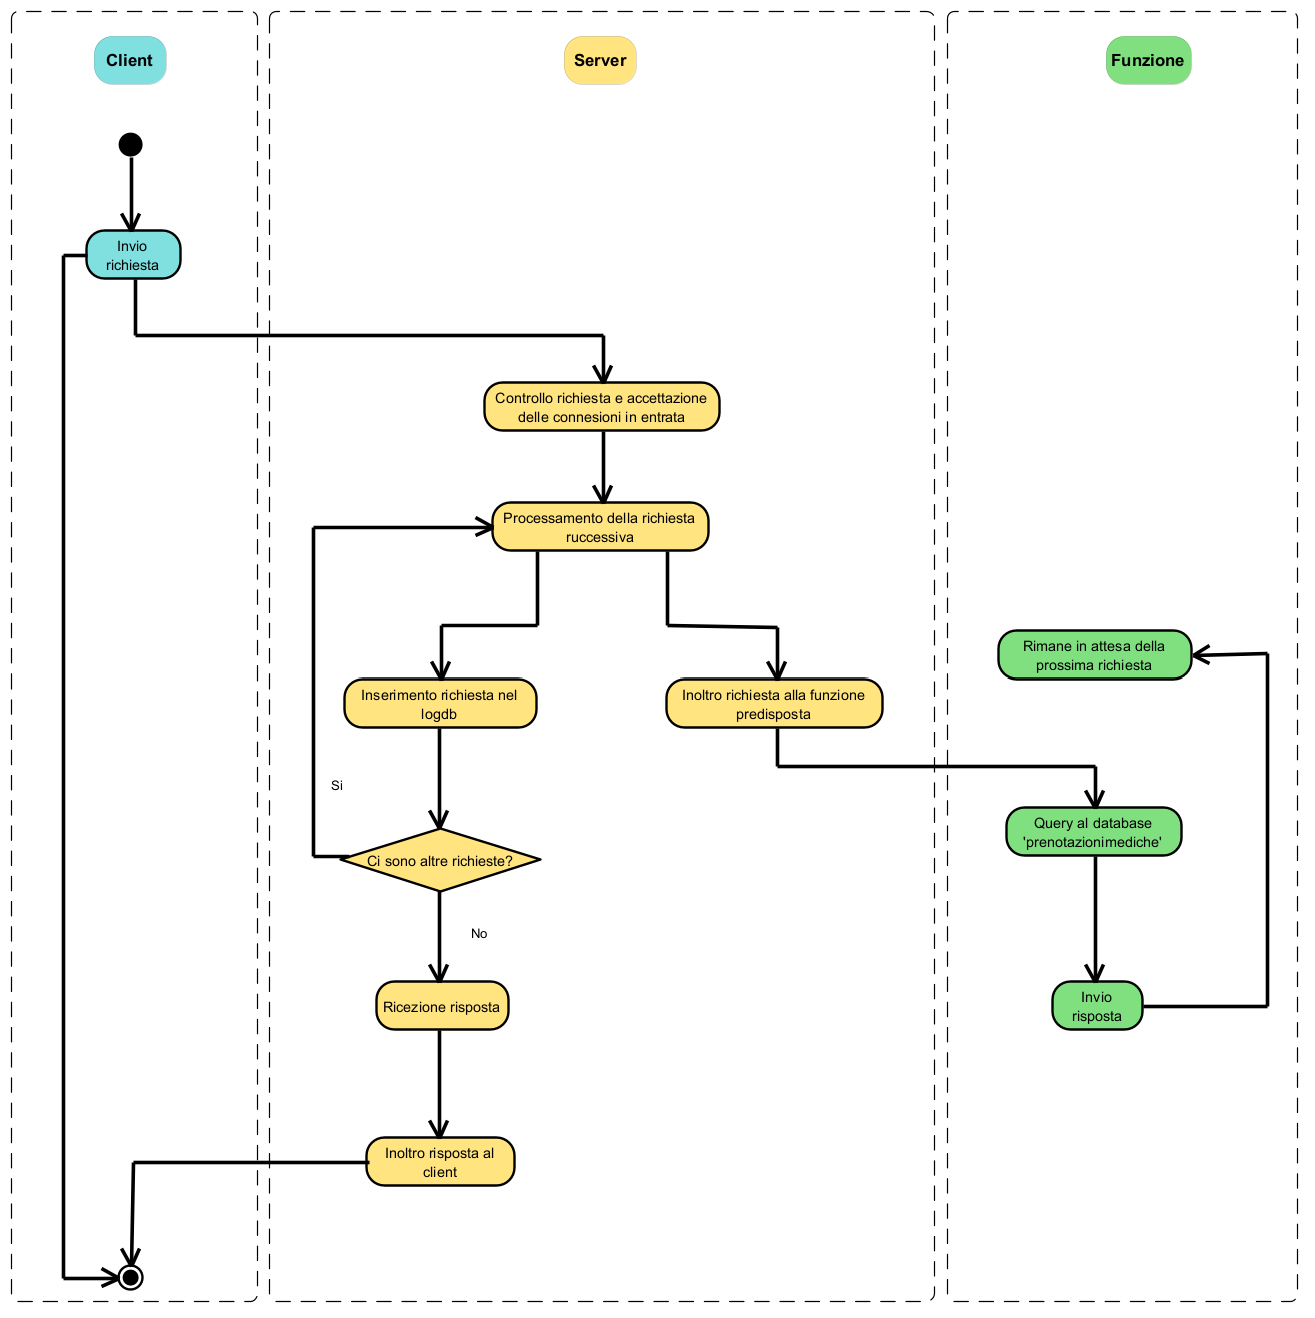
\includegraphics[width=1\linewidth]{images/Activity diagram.png}
        \label{Activity diagram}
    \end{figure}
    
    \subsection{State diagram}
    Tutte le Funzioni in esecuzione sui server sono come macchine a stati finiti, che alternano lo stato di ricezione, di elaborazione e d'invio della risposta.
    \begin{figure}[H]
        \centering
        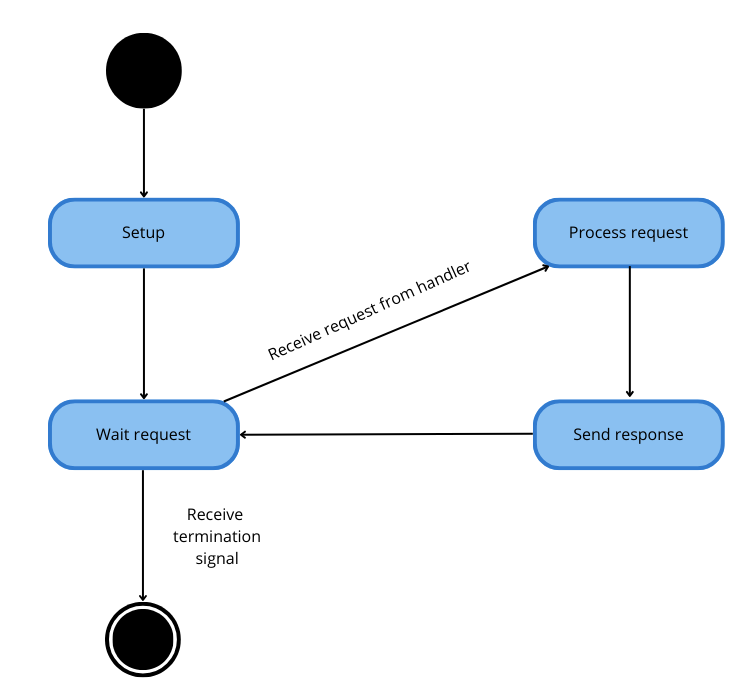
\includegraphics[width=0.5\linewidth]{images/StateDiagram1.png}
        \label{statediagram1}
    \end{figure}
    È importante notare come ogni Funzione rimane in esecuzione finché non viene ricevuto un segnale di terminazione da parte del server. Una volta ricevuto questo segnale ogni richiesta in esecuzione viene scartata senza comunicare il riscontro all'handler associato.\\
    Anche ognuno dei 4 server può essere visto come una macchina a stati finiti. A differenza delle Funzioni, però, i server non rimangono in attesa perenne di una richiesta, bensì, nel caso in cui non ce ne siano, procedono alla fase di controllo per eventuali risposte ricevute da parte delle proprie Funzioni.
    \begin{figure}[H]
        \centering
        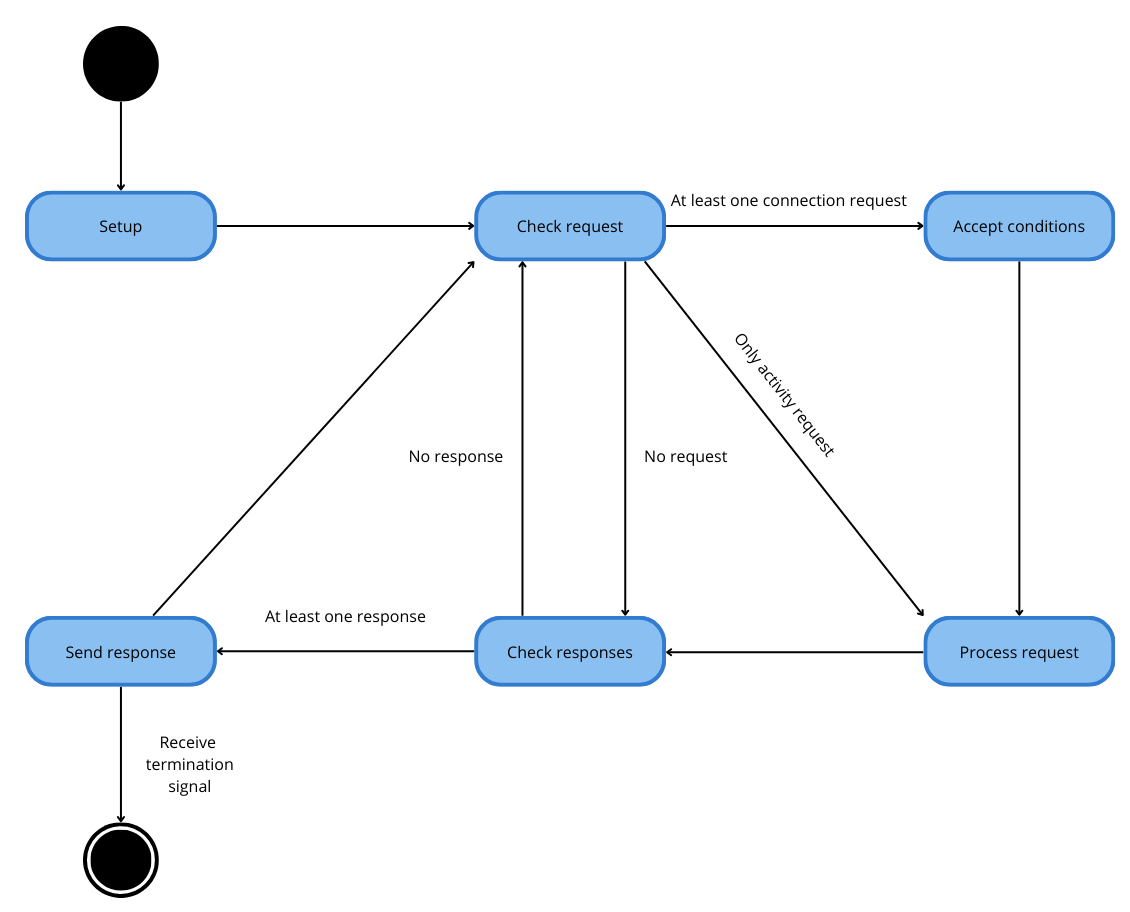
\includegraphics[width=0.5\linewidth]{images/StateDiagram2.png}
        \label{statediagram2}
    \end{figure}
    

    \subsection{Message Sequence Chart}
    Il message sequence chart rappresentato di seguito illustra l'invio di una richiesta da un client, la sua elaborazione e l'invio della risposta da parte del server. Come per gli Activity diagram, questo processo è comune a tutti i server e a tutte le loro funzioni, indipendentemente dal tipo di richiesta effettuata dal client. 
    \begin{figure}[H]
        \centering
        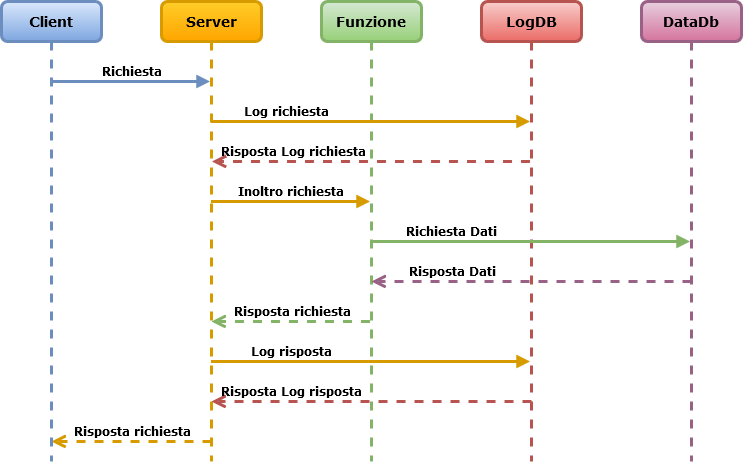
\includegraphics[width=1\linewidth]{images/MessageFlowChart.png}
        \label{Messageflowchart}
    \end{figure}
    

    \chapter{Implementazione del Software}
    
    \section{Struttura del codice}

    Il codice del nostro progetto è strutturato in varie cartelle:
    \subsection{db\_scripts}
    Nella cartella "db\_scripts" troviamo gli script che permettono l'inizializzazione e la creazione del database. Grazie ad essi è possibile creare il database che colleziona le entità del sistema, "prenotazionimediche" e il database che permette il controllo e la gestione delle connessioni "logdb".
    \subsection{src}
    Qui abbiamo la maggior parte degli script \textit{c++} che permettono la compilazione e l'esecuzione del progetto.
    
    Nello specifico:
    \begin{itemize}
        \item nella cartella "\textbf{classes}" troviamo tutte le classi utili allo svolgimento delle funzioni, la cartella
        \item in "\textbf{utils}" troviamo la funzione che permette alle varie funzionalità di sistema di inviare lo stato della risposta ricevuta dal database al client, oltre alle costanti di sistema
        \item la cartella "\textbf{server}"  definisce la struttura del server e dell'handler
        \item mentre nella cartella "\textbf{lib}" troviamo le librerie utilizzate per la connessione al database postgres e a redis.
    \end{itemize}   

    La struttura di ogni classe definita all'interno del sistema, ha il seguente schema:
        \lstset{
          language=C++, % Specifica il linguaggio C++
          basicstyle=\ttfamily\scriptsize, % Font per il codice (modificabile: \small, \scriptsize, ecc.)
          keywordstyle=\color{blue}, % Colore delle parole chiave
          stringstyle=\color{red}, % Colore per le stringhe
          commentstyle=\color{green!50!black}, % Colore per i commenti
          numberstyle=\tiny\color{gray}, % Font dei numeri di riga
          numbers=left, % Numeri di riga a sinistra
          stepnumber=1, % Numeri di riga ogni riga
          breaklines=true, % Ritorno a capo automatico
          breakatwhitespace=true, % Preferisce spezzare le righe negli spazi
          tabsize=4, % Dimensione dei tab
          frame=single, % Cornice attorno al codice
          captionpos=b, % Posizione della didascalia (b=bottom, t=top)
          showstringspaces=false % Non mostra spazi nelle stringhe
            }
    \begin{lstlisting}
#include "classeesempio.h"

ClasseEsempio::ClasseEsempio(char *id, char *campo_n2){
    this->id = (char *)malloc(sizeof(char) * PARAMETERS_LEN);
    this->campo_n2 = (char *)malloc(sizeof(char) * PARAMETERS_LEN);

    strcpy(this->id, id);
    strcpy(this->campo_n2,campo_n2 );
}

ClasseEsempio::~ClasseEsempio(){
    free(this->id);
    free(this->campo_n2);
}

ClasseEsempio *ClasseEsempio::from_stream(redisReply *reply, int stream_num, int msg_num){
    char key[PARAMETERS_LEN];
    char value[PARAMETERS_LEN];

    char id[PARAMETERS_LEN];
    char campo_n2[PARAMETERS_LEN];

    char read_fields = 0b00;

    for (int field_num = 2; field_num < ReadStreamMsgNumVal(reply, stream_num, msg_num); field_num += 2){
        ReadStreamMsgVal(reply, stream_num, msg_num, field_num, key);
        ReadStreamMsgVal(reply, stream_num, msg_num, field_num + 1, value);

        if (!strcmp(key, "id")){
            strcpy(id, value);
            read_fields |= 0b01;
        }
        else if (!strcmp(key, "campo_n2")){
            strcpy(campo_n2, value);
            read_fields |= 0b10;
        }
        else
        {
        throw std::invalid_argument("Stream error: invalid fields");
        }
    }

    if (read_fields != 0b11){
        throw std::invalid_argument("Stream error: invalid fields");
    }

    return new Amministrativo(id_amministrativo, cf_amministrativo);}
    \end{lstlisting}

    Sempre nella directory scr abbiamo poi altre 4 cartelle che definiscono le varie entità che possono svolgere azioni all'interno del sistema, troviamo infatti "\textbf{paziente\_non\_registrato}", "\textbf{paziente}", "\textbf{medico}", "\textbf{amministrativo}". All'interno di ognuna di queste vi è una struttura ben definita che suddivide le funzioni e l'handler all'interno di due cartelle separate.
    
    L'handler si occupa di istanziare un server dedicato e una volta che viene avviato direziona le richieste che gli giungono alle funzioni appartenenti alla propria entità.
    Le funzioni invece sono progettate per prendere in input gli stream dal flusso redis e utilizzarli o per fare query al database, o per creare oggetti, delle classi definite nella directory \textit{classes}. Le funzioni sono di due tipi, ovvero: le INSERT che prendono input da stream redis e che eseguono query al db per inserire dati, e le SELECT che invece prendono parametri da stream redis per cercare dati all'interno del database.

    Vediamo di seguito lo pseudocodice della Funzione "registrazione" utilizzata dai pazienti non registrati per appunto registrarsi al sistema di prenotazione:
    \begin{lstlisting}
INCLUDI "main.h"

funzione principale
    dichiara variabili di connessione Redis e risposte Redis
    dichiara variabile di risultato della query

    dichiara array per query, risposta, id del messaggio, prima chiave, id del client

    Inizializza connessione al database
    Inizializza connessione a Redis

    dichiara oggetti Persona e Paziente

    ciclo infinito
        leggi il comando Redis per il gruppo "main" e lo stream "paziente_non_registrato"
        
        verifica la risposta di Redis
        
        se non ci sono messaggi nello stream
            continua al prossimo ciclo

        leggi l ID del messaggio dallo stream

        leggi la prima chiave e l ID del client dallo stream

        se la prima chiave non e "client_id"
            invia la risposta con stato "BAD_REQUEST"
            continua al prossimo ciclo

        prova
            crea oggetti Persona e Paziente dallo stream
        se si verifica un eccezione
            invia la risposta con stato "BAD_REQUEST"
            stampa l errore
            continua al prossimo ciclo

        formatta la query SQL per inserire i dati di Persona e Paziente nel database

        esegui la query sul database

        se la query non e andata a buon fine
            invia la risposta con stato "DB_ERROR"
            continua al prossimo ciclo

        invia la risposta con stato "REQUEST_SUCCESS"

    chiudi la connessione al database

    ritorna 0

    \end{lstlisting}
    
    \subsection{tests}
    Nella cartella tests troviamo il test generator del sistema, il quale funzioan nel segueente modo: innanzitutto configura l'indirizzo ip  del server, e inizializza una lista per tenere traccia degli errori. Successivamente vengono generati valori casuali per un determinato parametro e viene generata una richiesta casuale, per ogni set di argomenti viene ritornata una stringa formattata di richiesta. Abbiamo poi la funzione \textbf{send\_request} che invia una richiesta al server utilizzando una connessione al socket. Una volta avviato il test generator abbiamo l'inizializzazione dei generatori di parametri casuali, la creazione di variabili casuali, l'invio della richiesta al server, viene poi restituita la risposta.
    
    
    \section{Descrizione connessioni Redis}
    In questo progetto viene utilizzato redis per inviare richieste al server che leggerà da stream e registrerà i dati all'interno delle classi, inoltre vengono inviati anche stream redis in output come risposta da parte del server per indicare al client i risultati delle query. 
    
    \section{Schema del database}
    \begin{figure}[H]
        \centering
        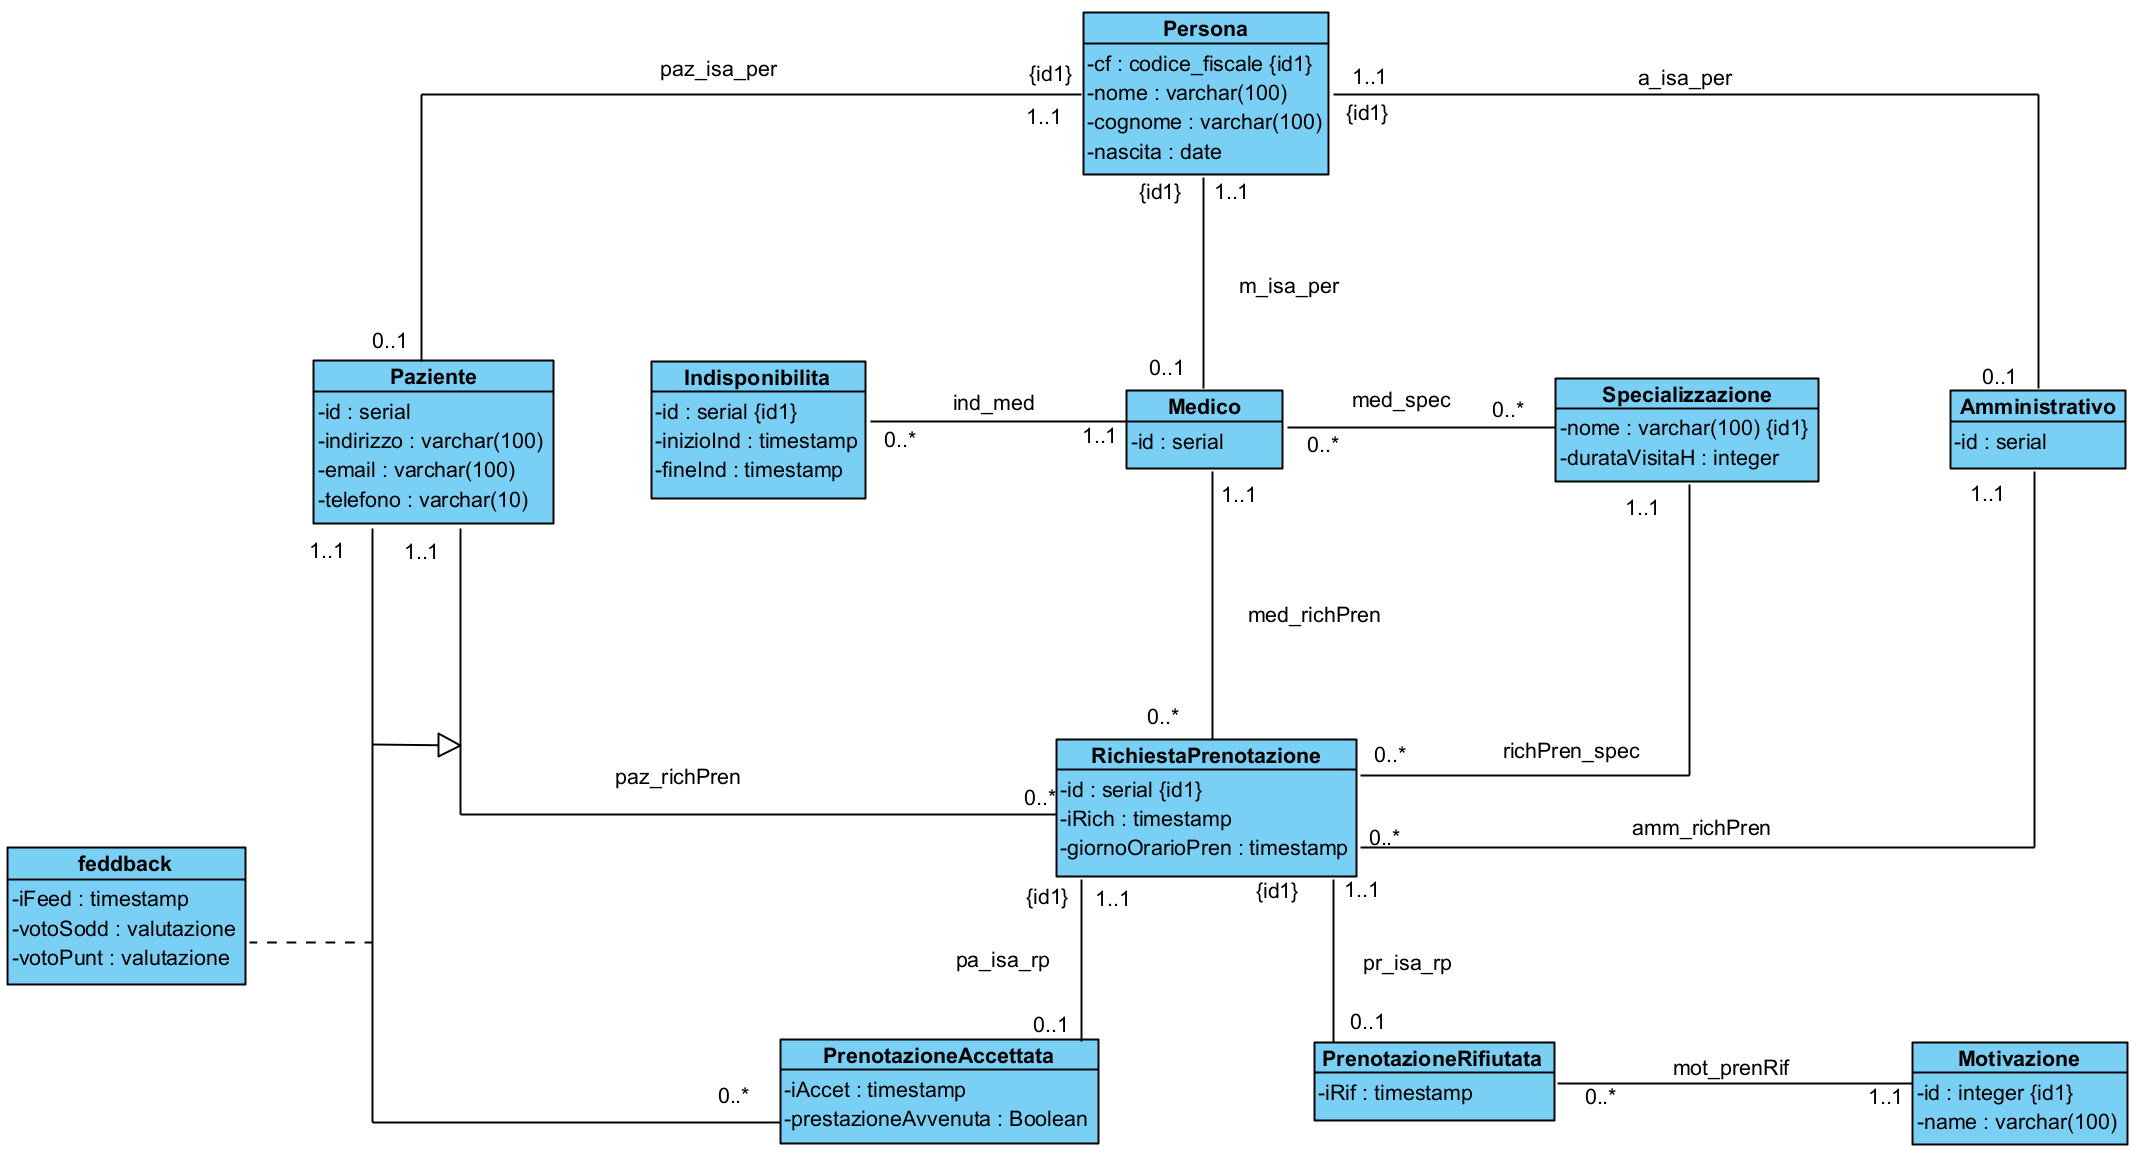
\includegraphics[width=1\linewidth]{images/UML prenotazionimediche ristrutturato.png}
        \label{UML prenotazionimediche ristrutturato}
    \end{figure}

    \newpage
    \section{Monitor funzionali}
    
    Nella realizzazione del database sono stati integrati vari monitor funzionali, realizzati mediante trigger. Questi operano come monitor attivi, prevenendo situazioni in cui i dati risultino inconsistenti tra loro, impedendo che vengano fatti INSERT, DELETE o UPDATE dal database che vadano a violare i vincoli esterni stabiliti durante il raffinamento dei requisiti, la creazione del diagramma UML e la sua ristrutturazione.

    Di seguito l'implementazion di tre trigger, presi come esempio:

    \begin{itemize}
    \item Trigger per la disgiunzione fra le richieste di prenotazione accettate e quelle rifiutate

    \lstset{
              language=SQL, % Imposta il linguaggio come SQL
              basicstyle=\ttfamily\scriptsize, % Font del codice (modificabile)
              keywordstyle=\color{blue}\bfseries, % Parole chiave in blu e in grassetto
              stringstyle=\color{red}, % Stringhe in rosso
              commentstyle=\color{green!50!black}, % Commenti in verde
              numberstyle=\tiny\color{gray}, % Numeri di riga piccoli e grigi
              numbers=left, % Numeri di riga a sinistra
              stepnumber=1, % Visualizza numeri ogni riga
              breaklines=true, % Abilita il ritorno a capo automatico
              breakatwhitespace=true, % Preferisce spezzare agli spazi
              tabsize=4, % Dimensione dei tab
              frame=single, % Cornice attorno al codice
              captionpos=b, % Posizione della didascalia (b=bottom, t=top)
              showstringspaces=false % Non mostra spazi nelle stringhe
            } 
    \begin{lstlisting}
-- [V.richiestaprenotazione.disgiunzione]
CREATE OR REPLACE FUNCTION verifica_disgiunzione_richiesta()
RETURNS TRIGGER AS $$
BEGIN
    IF TG_TABLE_NAME = 'prenotazioneaccettata' THEN
        IF EXISTS (
            SELECT 1 FROM prenotazionerifiutata WHERE richiesta_id = NEW.richiesta_id
        ) THEN
            RAISE EXCEPTION "Violazione del vincolo: La RichiestaPrenotazione e' gia' stata rifiutata";
        END IF;
    ELSIF TG_TABLE_NAME = 'prenotazionerifiutata' THEN
        IF EXISTS (
            SELECT 1 FROM prenotazioneaccettata WHERE richiesta_id = NEW.richiesta_id
        ) THEN
            RAISE EXCEPTION "Violazione del vincolo: La RichiestaPrenotazione e' gia' stata accettata";
        END IF;
    END IF;
    RETURN NEW;
END;
$$ LANGUAGE plpgsql;

CREATE TRIGGER trg_verifica_disgiunzione_accettata
BEFORE INSERT OR UPDATE ON prenotazioneaccettata
FOR EACH ROW
EXECUTE FUNCTION verifica_disgiunzione_richiesta();

CREATE TRIGGER trg_verifica_disgiunzione_rifiutata
BEFORE INSERT OR UPDATE ON prenotazionerifiutata
FOR EACH ROW
EXECUTE FUNCTION verifica_disgiunzione_richiesta();
    \end{lstlisting}
\newpage
    \item Trigger per la consistenza tra le richieste di prenotazione presenti nel sistema e quelle accettate o rifiutate dagli amministrativi

    \begin{lstlisting}
-- [V.prenotazioneaccettata/rifiutata.legale]
CREATE OR REPLACE FUNCTION controllo_richiesta_valida()
RETURNS TRIGGER AS $$
DECLARE
    richiesta RECORD;
BEGIN
    -- Recupera i dati della richiesta corrispondente
    SELECT irich, giornoorariopren
    INTO richiesta
    FROM richiestaprenotazione
    WHERE id = NEW.richiesta_id;

    -- Verifica che la richiesta esista
    IF NOT FOUND THEN
        RAISE EXCEPTION 'Violazione del vincolo: La prenotazione deve riferirsi a una richiesta valida';
    END IF;

    -- Logica per prenotazioneaccettata
    IF TG_TABLE_NAME = 'prenotazioneaccettata' THEN
        IF NOT (NEW.iaccet > richiesta.irich AND NEW.iaccet < richiesta.giornoorariopren) THEN
            RAISE EXCEPTION 'Violazione del vincolo: iaccett deve essere maggiore di irich e minore di giornoorariopren';
        END IF;

    -- Logica per prenotazionerifiutata
    ELSIF TG_TABLE_NAME = 'prenotazionerifiutata' THEN
        IF NOT (NEW.irif > richiesta.irich AND NEW.irif < richiesta.giornoorariopren) THEN
            RAISE EXCEPTION 'Violazione del vincolo: irif deve essere maggiore di irich e minore di giornoorariopren';
        END IF;
    END IF;

    RETURN NEW;
END;
$$ LANGUAGE plpgsql;

CREATE TRIGGER controllo_accettazione_valida
BEFORE INSERT OR UPDATE ON prenotazioneaccettata
FOR EACH ROW
EXECUTE FUNCTION controllo_richiesta_valida();

CREATE TRIGGER controllo_rifiuto_valido
BEFORE INSERT OR UPDATE ON prenotazionerifiutata
FOR EACH ROW
EXECUTE FUNCTION controllo_richiesta_valida();
    \end{lstlisting}
\newpage
    \item Trigger che controlla che un paziente lasci feedback solo su appuntamenti medici conclusi e da lui prenotati

    \begin{lstlisting}
CREATE OR REPLACE FUNCTION controllo_feedback_valido()
RETURNS TRIGGER AS $$
DECLARE
    prenotazione RECORD;
    paziente_richiesta INT;
BEGIN
    -- Recupera i dati della prenotazione accettata
    SELECT rp.giornoorariopren, pa.prestazioneavvenuta, rp.paziente_id
    INTO prenotazione
    FROM prenotazioneaccettata pa, richiestaprenotazione rp
    WHERE pa.richiesta_id = rp.id and pa.richiesta_id = NEW.prenotazione_accettata_id;

    -- Verifica che la prenotazione esista
    IF NOT FOUND THEN
        RAISE EXCEPTION 'Violazione del vincolo: Il feedback deve riferirsi a una prenotazione accettata valida.';
    END IF;

    -- Verifica che il paziente che sta lasciando il feedback sia lo stesso che ha fatto la prenotazione
    IF prenotazione.paziente_id != NEW.paziente_id THEN
        RAISE EXCEPTION 'Violazione del vincolo: Il paziente non corrisponde a quello che ha effettuato la prenotazione.';
    END IF;

    -- Verifica che la prestazione sia avvenuta
    IF prenotazione.prestazioneavvenuta = false THEN
        RAISE EXCEPTION 'Violazione del vincolo: La prestazione deve essere avvenuta prima di lasciare un feedback.';
    END IF;

    -- Verifica che ifeed sia maggiore di giornoorariopren
    IF NOT (NEW.ifeed > prenotazione.giornoorariopren) THEN
        RAISE EXCEPTION 'Violazione del vincolo: Il timestamp del feedback deve essere maggiore di giornoorariopren.';
    END IF;

    RETURN NEW;
END;
$$ LANGUAGE plpgsql;

CREATE TRIGGER controllo_feedback_valido
BEFORE INSERT OR UPDATE ON feedback
FOR EACH ROW
EXECUTE FUNCTION controllo_feedback_valido();
    \end{lstlisting}
        
    \end{itemize}

    \underline{\textbf{Nota}}: tutti gli altri trigger presenti nel databese possono essere visualizzati all'interno del file \texttt{db\_scripts/triggers.sql}.

    \newpage
    
    \section{Monitor non-funzionali}

\lstset{
          language=C++, % Specifica il linguaggio C++
          basicstyle=\ttfamily\scriptsize, % Font per il codice (modificabile: \small, \scriptsize, ecc.)
          keywordstyle=\color{blue}, % Colore delle parole chiave
          stringstyle=\color{red}, % Colore per le stringhe
          commentstyle=\color{green!50!black}, % Colore per i commenti
          numberstyle=\tiny\color{gray}, % Font dei numeri di riga
          numbers=left, % Numeri di riga a sinistra
          stepnumber=1, % Numeri di riga ogni riga
          breaklines=true, % Ritorno a capo automatico
          breakatwhitespace=true, % Preferisce spezzare le righe negli spazi
          tabsize=4, % Dimensione dei tab
          frame=single, % Cornice attorno al codice
          captionpos=b, % Posizione della didascalia (b=bottom, t=top)
          showstringspaces=false % Non mostra spazi nelle stringhe
            }
\begin{lstlisting}
while(true) {
    query = "
        SELECT EXTRACT(
            EPOCH FROM AVG(idisconnection - iconnection)
        ) * 1000 as avg
        FROM Client
        WHERE idisconnection IS NOT NULL
    ";

    average = log_db.execQuery(query);

    if average <= MAX_CONNECTION_TIME_AVG:
        responseStatus = "SUCCESS";
    else:
        responseStatus = "ERROR";

    query = "
        INSERT INTO
        SessionStatistic(type, iend, value, response_status)
        VALUES ('Session', CURRENT_TIMESTAMP, average, responseStatus)
    ";

    log_db.execQuery(query);

    query = "
        SELECT EXTRACT(
            EPOCH FROM AVG(iresponse - irequest)
        ) * 1000 as avg
        FROM Communication
        WHERE iresponse IS NOT NULL
    ";

    average = log_db.checkQueryResult(query);

    
    if average <= MAX_RESPONSE_TIME_AVG:
        responseStatus = "SUCCESS";
    else:
        responseStatus = "ERROR";

    query = "
        INSERT INTO
        SessionStatistic(type, iend, value, response_status)
        VALUES ('Response', CURRENT_TIMESTAMP, average, responseStatus)
    ";

    log_db.execQuery(query);

    sleep(60sec);
}

\end{lstlisting}

\section{Risultati Sperimentali}
    Il progetto, nel suo complesso, rappresenta una piattaforma di prenotazioni mediche conforme agli standard moderni. I risultati ottenuti attraverso il test generator dimostrano che la piattaforma è in grado di adempiere efficacemente alle sue finalità, gestendo in modo semplice ed efficiente le prenotazioni ospedaliere sia per i pazienti che per il personale amministrativo. Inoltre, i test hanno evidenziato la capacità della piattaforma di affrontare eventuali sovraccarichi di richieste, grazie alla gestione parallela delle operazioni e alla capacità di gestire eventuali errori che possono verificarsi durante le richieste.  

\end{document}